\section{Datasets Utilizados}
\label{sec:datasets_utilizados}

A concepção, o treinamento e a validação empírica de Sistemas de Detecção de Intrusão em Redes (\emph{Network Intrusion Detection Systems} -- NIDS) orientados a Aprendizado de Máquina e Aprendizado Profundo são diretamente condicionados pela qualidade, diversidade e representatividade dos conjuntos de dados empregados \cite{standard2021, netflow2020}. Historicamente, a comunidade de segurança da informação recorreu a bases públicas pioneiras, tais como DARPA~98, KDD~Cup~99 e NSL-KDD. Não obstante a sua relevância histórica, tais bases tornaram-se anacrônicas face às transformações da Internet contemporânea: exibem tráfego artificial gerado em ambientes desprovidos de ruído operacional humano, não contemplam protocolos criptografados e contêm distribuições estatísticas que não reproduzem a complexidade e a volumetria das ameaças atuais \cite{Sharafaldin2018TowardGA, advancedids2024}.

Com o intuito de superar tais deficiências metodológicas e assegurar que os modelos avaliados operem sob condições operacionais fidedignas, este trabalho adota o paradigma de análise fundamentado em fluxos de rede bidirecionais (\emph{bidirectional network flows}). Formalmente, um fluxo de rede $\mathcal{F}$ é definido como uma sequência temporal de pacotes de dados transmitidos entre dois nós terminais ao longo de um canal de comunicação, unicamente indexados pela tupla quíntupla de cabeçalho L3/L4 (\emph{5-tuple}):
\begin{equation}
\label{eq:fluxo_definicao}
\mathcal{F} = \langle IP_{\mathrm{orig}}, Port_{\mathrm{orig}}, IP_{\mathrm{dest}}, Port_{\mathrm{dest}}, Prot \rangle,
\end{equation}
em que $IP_{\mathrm{orig}}$ e $IP_{\mathrm{dest}}$ denotam os endereços de Protocolo de Internet (\emph{Internet Protocol} -- IP) de origem e destino, $Port_{\mathrm{orig}}$ e $Port_{\mathrm{dest}}$ correspondem às portas da camada de transporte (TCP ou UDP), e $Prot$ identifica o protocolo encapsulado ($Prot \in \{6 \text{ (TCP)}, 17 \text{ (UDP)}, \dots\}$).

A delimitação temporal de um fluxo é regida por duas variáveis fundamentais de controle:
\begin{enumerate}
    \item \textbf{Tempo de Inatividade (\emph{Idle Timeout} -- $\tau_{\mathrm{idle}}$):} intervalo temporal máximo admissível de ausência de transmissão entre os interlocutores (comumente parametrizado em $120\,\mathrm{s}$); caso superado, o fluxo é encerrado e exportado para sumarização estatística;
    \item \textbf{Tempo Máximo Ativo (\emph{Active Timeout} -- $\tau_{\mathrm{active}}$):} limiar superior de duração total concedido a uma conexão contínua em trânsito (padronizado em $1800\,\mathrm{s}$ nas especificações clássicas de NetFlow/IPFIX, mas especificamente configurado para $\tau_{\mathrm{active}} = 240\,\mathrm{s}$ no ambiente experimental deste trabalho); atingido esse limite, o fluxo é segmentado e consolidado para viabilizar a inspeção periódica de conexões persistentes de longa duração e prevenir a retenção indefinida de estados na memória volátil dos monitores de rede sob ataques contínuos de negação de serviço.
\end{enumerate}

A partir do encerramento de um fluxo $\mathcal{F}$, ferramentas especializadas de extração estatística aplicam operadores de agregação sobre as distribuições de tempo, tamanho e sinalizadores, gerando um vetor de atributos numéricos $\mathbf{x} \in \mathbb{R}^D$:
\begin{equation}
\label{eq:vetor_caracteristicas}
\mathbf{x} = \phi(\mathcal{F}) = [f_1, f_2, \dots, f_D]^T,
\end{equation}
sendo $\phi(\cdot)$ a função de mapeamento implementada pelo extrator de telemetria e $D$ a dimensionalidade do vetor característico.

Neste trabalho, são selecionados conjuntos de dados consolidados e complementares que cobrem diferentes espectros de tráfego, topologias e vetores de ameaça:
\begin{itemize}
    \item \textbf{CSE-CIC-IDS2018 (Versão Canônica e Versão Corrigida):} referência consagrada para tráfego corporativo e ataques complexos distribuídos em infraestrutura de nuvem AWS, avaliada tanto em sua rotulação original (15 classes brutas) quanto sob a auditoria sistemática de \citeonline{liu2022error} (25 classes originais reclassificadas em 15 classes efetivas e 9 macro-famílias);
    \item \textbf{CIC-BCCC-NRC TabularIoTAttack-2024:} \emph{benchmark} contemporâneo consolidado a partir da integração de 9 sub-datasets de Internet das Coisas (\emph{Internet of Things} -- IoT), contemplando protocolos leves de telemetria (MQTT) e variantes modernas de negação de serviço e botnets (49 classes granulares e 9 macro-famílias);
    \item \textbf{CIC-UNSW-NB15:} base de referência analítica contendo tráfego sintético e realístico de alta densidade gerado por hardware dedicado de emulação (IXIA PerfectStorm), estruturada em 10 classes e processada via amostragem com entropia comportamental.
\end{itemize}

O \ref{quadro:comparativo_geral_datasets} sintetiza as propriedades fundamentais, origens e características operacionais dos conjuntos de dados analisados nesta pesquisa.

\begin{quadro}[htb]
\centering
\caption{Síntese comparativa dos conjuntos de dados selecionados para treinamento e avaliação.}
\label{quadro:comparativo_geral_datasets}
\footnotesize
\setlength{\tabcolsep}{4pt}
\renewcommand{\arraystretch}{1.2}
\begin{tabularx}{\textwidth}{|>{\raggedright\arraybackslash}p{2.6cm}|c|>{\raggedright\arraybackslash}X|>{\raggedright\arraybackslash}X|>{\centering\arraybackslash}p{2.3cm}|>{\centering\arraybackslash}p{2.0cm}|}
\hline
\textbf{Dataset} & \textbf{Ano} & \textbf{Ambiente de Captura} & \textbf{Mecanismo de Geração} & \textbf{Atributos} & \textbf{Classes} \\ \hline
CSE-CIC-IDS2018\newline(Original) & 2018 & Nuvem AWS corporativa (5 departamentos e \emph{server room}) & Agentes B-Profile (humanos) e M-Profiles (ataques) & 80 $\to$ 76\newline(73 ativas) & 15 (L0) \slash\newline 7 (L2) \\ \hline
CSE-CIC-IDS2018\newline(Corrigido) & 2022 & Nuvem AWS corporativa (auditoria Liu et al., 2022) & Reclassificação de fluxos com portas fechadas\slash tentativas & 91 $\to$ 81 $\to$ 76\newline(73 ativas) & 15 (25 orig.) \slash\newline 9 (L2) \\ \hline
CIC-BCCC-NRC\newline TabularIoTAttack-2024 & 2024 & Laboratórios físicos e híbridos IoT\slash IoMT (IoTRL e UNB) & Produto de 9 sub-datasets (sensores, MQTT e rotinas) & 85 $\to$ 71\newline(73 ativas) & 49 (L0) \slash\newline 9 (L2) \\ \hline
CIC-UNSW-NB15 & 2015 & Cyber Range Lab (ACCS\slash UNSW Canberra) & Dispositivo IXIA PerfectStorm e tráfego realístico & 84 $\to$ 75\newline(73 ativas) & 10 (L0) \\ \hline
\end{tabularx}
\fonte{Elaborado pelo autor (2026).}
\end{quadro}


\subsection{CSE-CIC-IDS2018: Versão Canônica e Versão Corrigida}
\label{subsec:cse_cic_ids2018}

O conjunto de dados CSE-CIC-IDS2018 (\emph{Communications Security Establishment \& Canadian Institute for Cybersecurity}) foi desenvolvido mediante um projeto de cooperação técnica entre o instituto governamental canadense Communications Security Establishment e o Canadian Institute for Cybersecurity da University of New Brunswick (UNB) \cite{Sharafaldin2018TowardGA}. O objetivo consistiu na criação de um repositório de segurança cibernética em grande escala, hospedado na plataforma Amazon Web Services (AWS), superando as restrições de anonimização excessiva e volume diminuto presentes em bases legadas.

\subsubsection{Topologia e Infraestrutura de Rede}

A concepção experimental do CSE-CIC-IDS2018 compreendeu duas redes completamente divididas: a Rede da Vítima (\emph{Victim-Network}) e a Rede de Ataque (\emph{Attack-Network}). A \emph{Victim-Network} replica a infraestrutura de uma organização corporativa de médio e grande porte, estruturada em cinco departamentos operacionais independentes conectados a uma sala de servidores (\emph{Server Room}):
\begin{itemize}
    \item \textbf{Controladora de Domínio e Infraestrutura Central:} servidor Windows Server 2016 desempenhando funções de Diretório Ativo (\emph{Active Directory}), DNS e autenticação centralizada;
    \item \textbf{Servidores de Aplicação:} servidores com Ubuntu Linux (versões 12, 14.04 e 16.04) hospedando serviços web HTTP/HTTPS, bancos de dados relacionais e servidores FTP;
    \item \textbf{Estações de Trabalho Heterogêneas:} mais de 500 máquinas clientes conectadas à rede interna, englobando Windows~10, Windows~8.1, Windows~7, distribuições Linux e macOS;
    \item \textbf{Dispositivos de Interconexão:} firewalls corporativos (Fortinet) e switches gerenciáveis com espelhamento de portas (\emph{port mirroring}), viabilizando a gravação sem perdas de tráfego bruto em PCAP.
\end{itemize}

A \emph{Attack-Network} abrangeu cerca de 50 estações atacantes operando Kali Linux e Windows~8.1 na AWS, provisionadas com endereçamento IP público e conectividade direta com o perímetro corporativo alvo.

\subsubsection{Metodologia de Geração de Tráfego e Limitações Metodológicas do Estado da Arte}

A geração de tráfego empregou dois perfis comportamentais \cite{Sharafaldin2018TowardGA}: o \emph{B-Profile} (agente em Java modelando interações humanas realísticas em HTTP, HTTPS, FTP, SSH e e-mail) e o \emph{M-Profile} (rotinas automatizadas de agressão abrangendo ataques de força bruta, Heartbleed, botnet Ares, DoS volumétrico/lento, DDoS via LOIC/HOIC, ataques web e infiltração em duas fases).

Entretanto, investigações recentes conduzidas por \citeonline{liu2022error} identificaram falhas sistemáticas e catastróficas de rotulação no CSE-CIC-IDS2018. Especificamente, constatou-se que o processo de etiquetagem original rotulou fluxos inteiros com base unicamente na janela temporal programada para a execução dos scripts de ataque, independentemente de os pacotes maliciosos terem efetivamente alcançado o serviço ou exibido comportamento anômalo. Dentre as inconsistências mais graves documentadas por \citeonline{liu2022error}, destacam-se:
\begin{enumerate}
    \item \textbf{Inconsistência em Ataques de Força Bruta FTP (\emph{FTP-BruteForce}):} Em ambos os dias de coleta em que o ataque foi supostamente desferido, o servidor alvo na porta 21 respondeu invariavelmente com pacotes sinalizados com \texttt{[RST, ACK]}. Esse padrão de sinalização comprova que a porta do serviço estava fechada no sistema operacional de destino; logo, o servidor rejeitou sumariamente a conexão, não ocorrendo qualquer interação de autenticação ou exploração. Portanto, rotular tais fluxos como ataque induz o modelo a aprender respostas legítimas de rejeição de porta TCP fechada como assinaturas maliciosas;
    \item \textbf{Superestimação de Categorias de Tentativa (\emph{Attempted Categories}):} Milhares de conexões foram marcadas como ataques consumados quando, na realidade, consistiam em simples tentativas inócuas ou ruído de fundo. No esquema original de \citeonline{liu2022error}, a auditoria catalogou inicialmente 25 categorias distintas (10 classes de tentativa, 14 classes de ataque efetivo e a classe Benign). Conforme demonstrado pelos autores, fluxos com o atributo \emph{Attempted Category} diferente de $-1$ devem ser consolidados como tráfego benigno (\emph{Benign}) para evitar o fenômeno de aprendizado espúrio (\emph{Garbage In, Garbage Out}), reduzindo o espaço alvo efetivo para 15 classes ativas no nível L0 e 9 macro-famílias no nível L2;
    \item \textbf{Desagregação Realista de Infiltração:} Na versão original, a classe \emph{Infilteration} agregou de forma indiferenciada varreduras de porta, transferências de arquivos e comunicação interna de comando e controle. A versão corrigida individualiza tais vetores em \emph{Infiltration - NMAP Portscan}, \emph{Infiltration - Dropbox Download} e \emph{Infiltration - Communication Victim Attacker};
    \item \textbf{Harmonização e Redução Dimensional:} Enquanto a versão original do CSE-CIC-IDS2018 disponibilizou 80 atributos brutos que resultam em 76 colunas canônicas (73 ativas após o expurgo de sinalizadores sem variância), a auditoria de \citeonline{liu2022error} partiu de 91 atributos brutos, destilou 81 métricas estatísticas de fluxo e foi harmonizada no mesmo espaço canônico de 76 atributos (73 ativos) adotado nesta tese.
\end{enumerate}

\subsubsection{Distribuição Amostral: Canônica vs. Corrigida}

Diante desse panorama metodológico, este trabalho adota uma estratégia analítica bifurcada: avalia-se o modelo ALF-MoE na base canônica (com 100\% dos fluxos de ataque originais e 10\% de benigno, totalizando 3.712.942 fluxos sem duplicatas, distribuídos em 15 classes e 7 macro-famílias) e, em paralelo, na base saneada com as correções de \citeonline{liu2022error} (consolidando 15 classes efetivas e 9 macro-famílias). A partição de teste (20\% estratificado) da versão canônica conta com 742.589 instâncias, enquanto a versão corrigida consolida 1.263.903 instâncias de teste. A Tabela~\ref{tab:distribuicao_csecicids2018_comparativa} contrasta as distribuições de teste observadas em ambas as variantes.

\begin{table}[htb]
\centering
\caption{Distribuição de classes e suporte amostral de teste: CSE-CIC-IDS2018 Canônico vs. Corrigido.}
\label{tab:distribuicao_csecicids2018_comparativa}
\footnotesize
\begin{tabularx}{\textwidth}{>{\raggedright\arraybackslash}Xrr >{\raggedright\arraybackslash}Xrr}
\hline
\multicolumn{3}{c}{\textbf{Versão Canônica (Original)}} & \multicolumn{3}{c}{\textbf{Versão Corrigida (Liu et al., 2022)}} \\
\textbf{Classe Canônica} & \textbf{Suporte} & \textbf{Proporção} & \textbf{Classe Corrigida} & \textbf{Suporte} & \textbf{Proporção} \\
\hline
Benign & 269.694 & 36,32\% & BENIGN & 1.128.279 & 89,27\% \\
Bot & 56.462 & 7,60\% & Botnet Ares & 28.584 & 2,26\% \\
Brute Force -Web & 122 & 0,02\% & Web Attack - Brute Force & 26 & 0,002\% \\
Brute Force -XSS & 46 & 0,01\% & Web Attack - XSS & 23 & 0,002\% \\
DDOS attack-HOIC & 133.693 & 18,00\% & DDoS-HOIC & 21.646 & 1,71\% \\
DDOS attack-LOIC-UDP & 346 & 0,05\% & DDoS-LOIC-UDP & 505 & 0,04\% \\
DDoS attacks-LOIC-HTTP & 115.235 & 15,52\% & DDoS-LOIC-HTTP & 5.787 & 0,46\% \\
DoS attacks-GoldenEye & 8.291 & 1,12\% & DoS GoldenEye & 4.512 & 0,36\% \\
DoS attacks-Hulk & 86.976 & 11,71\% & DoS Hulk & 36.063 & 2,85\% \\
DoS attacks-SlowHTTPTest & 5.935 & 0,80\% & -- (Reclassificado Benign) & -- & -- \\
DoS attacks-Slowloris & 2.057 & 0,28\% & DoS Slowloris & 1.698 & 0,13\% \\
FTP-BruteForce & 7.870 & 1,06\% & -- (Reclassificado Benign) & -- & -- \\
Infilteration & 32.380 & 4,36\% & Infiltration - NMAP Portscan & 17.875 & 1,41\% \\
-- & -- & -- & Infiltration - Comm. Victim & 41 & 0,003\% \\
-- & -- & -- & Infiltration - Dropbox & 17 & 0,001\% \\
SQL Injection & 17 & 0,002\% & Web Attack - SQL & 8 & 0,001\% \\
SSH-Bruteforce & 23.465 & 3,16\% & SSH-BruteForce & 18.839 & 1,49\% \\
\hline
\textbf{Total de Teste} & \textbf{742.589} & \textbf{100,00\%} & \textbf{Total de Teste} & \textbf{1.263.903} & \textbf{100,00\%} \\
\hline
\end{tabularx}
\fonte{Elaborado pelo autor (2026), com base em \citeonline{Sharafaldin2018TowardGA} e \citeonline{liu2022error}.}
\end{table}


\subsection{CIC-BCCC-NRC TabularIoTAttack-2024: Origem, Geração, Atributos e Distribuição Amostral}
\label{subsec:cic_bccc_nrc_2024}

A proliferação ubíqua de sensores e atuadores em ambientes industriais e residenciais ampliou substancialmente a superfície de ataque exposta a ameaças em ecossistemas de Internet das Coisas (\emph{Internet of Things} -- IoT) \cite{ciciot2023}. O tráfego de redes IoT exibe dinâmicas específicas: mensagens curtas assíncronas, protocolos de transporte e aplicação leves (tais como MQTT e CoAP) e restrições energéticas e computacionais severas nos nós de borda.

Para refletir essa realidade operacional, o Canadian Institute for Cybersecurity (CIC), o Bell Centre for Cyber Security (BCCC) e o National Research Council Canada (NRC) desenvolveram a base \emph{CIC-BCCC-NRC TabularIoTAttack-2024} \cite{sasi2025efficient}, concebida a partir da consolidação de 9 sub-datasets de telemetria de rede. O ambiente experimental combinou os laboratórios \emph{Internet of Things Research Lab} (IoTRL) do Army Cyber Institute e as bancadas do CIC/UNB, integrando mais de 40 dispositivos físicos (sensores, atuadores, câmeras IP, termostatos e comutadores sob protocolos IEEE~802.11, Zigbee, Z-Wave e BLE), concentradores Home Assistant, intermediadores MQTT e pontos de captura não invasiva via \emph{network taps} com \texttt{dumpcap}.

\subsubsection{Amostragem Estratificada Hare-Niemeyer e Distribuição Amostral}

Em decorrência da volumetria massiva da base completa e com o propósito de manter a viabilidade computacional sem comprometer a representatividade de eventos raros, adotou-se um protocolo de amostragem representativa de 15\% do volume total. A base bruta compreende 85 colunas originais, das quais 71 atributos estatísticos de fluxo foram mantidos na amostragem e compatibilizados com o vetor canônico de 73 atributos ativos do modelo. A metodologia preservou integralmente (100\% de retenção) todas as 14 classes de ataque raras presentes no banco e aplicou o método de alocação de maiores restos de \emph{Hare-Niemeyer} nas 35 classes majoritárias restantes.

A partição de teste resultante consolidou 652.845 fluxos de rede. No nível granular (Threat Level 0), o conjunto engloba 49 classes ativas, compreendendo inundações volumétricas, fragmentações maliciosas de datagramas L3/L4 (\emph{DDoS ACK Fragmentation}, \emph{DDoS ICMP Fragmentation}), explorações do protocolo MQTT (\emph{MQTT Connect Flood}, \emph{Publish Flood}, \emph{Malformed}), variantes de botnet Mirai, varreduras ativas e ataques de autenticação, estruturadas em 9 macro-famílias funcionais no nível L2. A Tabela~\ref{tab:distribuicao_cicbccc2024_resumida} sumariza o suporte amostral das classes no conjunto de teste.

\begin{table}[htb]
\centering
\caption{Macro-famílias e distribuição amostral de teste no benchmark CIC-BCCC-NRC TabularIoTAttack-2024.}
\label{tab:distribuicao_cicbccc2024_resumida}
\small
\begin{tabularx}{\textwidth}{lXrr}
\hline
\textbf{Macro-Família (L2)} & \textbf{Principais Classes Granulares (L0)} & \textbf{Suporte} & \textbf{Proporção} \\
\hline
Benign Traffic & Benign Traffic (70.185) & 70.185 & 10,75\% \\
Botnet / Malware & Backdoor (12.127), Mirai Variants (2.068), Ransomware (496) & 14.691 & 2,25\% \\
BruteForce & Sparta SSH (33.430), Password Attack (5.335), Dictionary (540), Telnet (138) & 39.443 & 6,04\% \\
DDoS & DDoS RSTFIN (117.262), DDoS PSHACK (75.840), DDoS ACK Frag (12.083), Outros & 207.074 & 31,72\% \\
DoS & ACK Flood (86.511), DoS TCP Flood (66.891), SYN Flood (53.713), Outros & 211.296 & 32,37\% \\
IoT / MQTT & MQTT Brute Force (30.249), MQTT DDoS Publish (12.324), MQTT DoS (7.278), Outros & 50.282 & 7,70\% \\
MITM & MITM (3.278), MITM ARP Spoofing (515) & 3.793 & 0,58\% \\
Reconnaissance & Recon Port Scan (25.795), Recon OS Scan (3.796), Ping Sweep, Host Discovery, etc. & 34.461 & 5,28\% \\
WebAttack & XSS (21.076), Uploading Attack (283), SQL Injection (261) & 21.620 & 3,31\% \\
\hline
\textbf{Total Avaliado} & \textbf{49 Classes Granulares Consolidadas em 9 Macro-Famílias} & \textbf{652.845} & \textbf{100,00\%} \\
\hline
\end{tabularx}
\fonte{Elaborado pelo autor (2026), com base em \citeonline{sasi2025efficient}.}
\end{table}


\subsection{CIC-UNSW-NB15: Origem, Geração, Atributos e Distribuição Amostral}
\label{subsec:unsw_nb15}

O conjunto de dados UNSW-NB15 foi concebido em 2015 pelo \emph{Cyber Range Lab} do \emph{Australian Centre for Cyber Security} (ACCS), na Universidade de New South Wales \cite{moustafa2015unsw, standard2021}. A geração baseou-se na plataforma de hardware dedicada \textbf{IXIA PerfectStorm}, injetando tráfego sintético contemporâneo e tráfego de fundo operacional realístico em canais Gigabit Ethernet, totalizando 100~GB de tráfego bruto capturado em formato PCAP.

Para harmonizar o espaço de entrada entre os múltiplos especialistas da arquitetura ALF-MoE, este trabalho adota a versão extraída via motor CICFlowMeter, designada \emph{CIC-UNSW-NB15}. A base abrange originalmente 84 atributos brutos que, após o expurgo de identificadores de socket, colinearidades exatas e variáveis de variância nula, resultam em 75 atributos estatísticos, diretamente alinhados ao vetor de 73 atributos ativos do modelo. Em termos de taxonomia, a base abrange nove famílias de ataques cibernéticos e o tráfego legítimo (\emph{Benign}): \emph{Analysis}, \emph{Backdoor}, \emph{DoS}, \emph{Exploits}, \emph{Fuzzers}, \emph{Generic}, \emph{Reconnaissance}, \emph{Shellcode} e \emph{Worms}.

\subsubsection{Mitigação de GIGO e Amostragem com Máxima Entropia}

Na análise exploratória inicial da base CIC-UNSW-NB15, constatou-se uma discrepância volumétrica extrema entre as classes maliciosas e os fluxos normais redundantes. Para prevenir o viés de super-representação e degradação por GIGO, formulou-se um pipeline de amostragem estratificada multivariada: preservou-se 100\% dos fluxos de ataque disponíveis e realizou-se a seleção das 50.000 instâncias benignas mais informativas com base no critério de máxima cobertura comportamental e entropia no espaço de atributos.

Após a subsequente desduplicação exata de fluxos idênticos, a base consolidou 125.378 instâncias, distribuídas na proporção 80\% para desenvolvimento (80.241 treino, 20.061 validação) e 20\% para teste independente (27.917 fluxos). A Tabela~\ref{tab:distribuicao_unswnb15_real} apresenta o suporte de teste para as dez classes.

\begin{table}[htb]
\centering
\caption{Distribuição de classes e suporte amostral no benchmark CIC-UNSW-NB15.}
\label{tab:distribuicao_unswnb15_real}
\small
\begin{tabularx}{\textwidth}{cl>{\raggedright\arraybackslash}Xrr}
\hline
\textbf{ID} & \textbf{Classe Canônica} & \textbf{Vetor de Ameaça} & \textbf{Amostras (Teste)} & \textbf{Proporção (\%)} \\
\hline
0 & Analysis & Varreduras pontuais de diretórios e sondagem HTTP & 77 & 0,28\% \\
1 & Backdoor & Canais de acesso furtivo e persistência em nós comprometidos & 90 & 0,32\% \\
2 & Benign & Conexões legítimas de rede corporativa e navegação & 10.000 & 35,82\% \\
3 & DoS & Esgotamento de buffers e saturação de largura de banda & 894 & 3,20\% \\
4 & Exploits & Exploração direta de vulnerabilidades registradas (CVE) & 6.190 & 22,17\% \\
5 & Fuzzers & Injeção de cargas corrompidas para indução de falhas & 5.923 & 21,22\% \\
6 & Generic & Colisões criptográficas e ataques genéricos de cifras & 927 & 3,32\% \\
7 & Reconnaissance & Mapeamento de topologia e enumeração de serviços ativos & 3.347 & 11,99\% \\
8 & Shellcode & Payloads binários para invocação de shell privilegiada & 420 & 1,50\% \\
9 & Worms & Códigos maliciosos com propagação e replicação autônoma & 49 & 0,18\% \\
\hline
\multicolumn{3}{l}{\textbf{Total de Instâncias Avaliadas}} & \textbf{27.917} & \textbf{100,00\%} \\
\hline
\end{tabularx}
\fonte{Elaborado pelo autor (2026), com base em metadados de execução.}
\end{table}


\subsection{Modelagem de Hierarquia de Ameaças (\emph{Threat Levels})}
\label{subsec:threat_levels}

Em operações reais de cibersegurança em Centros de Operações de Segurança (\emph{Security Operations Centers} -- SOC), a resposta a incidentes demanda diferentes níveis de abstração semântica:
\begin{itemize}
    \item \textbf{Nível de Ameaça 0 (\emph{Threat Level 0} -- Granularidade Estrita):} Mantém as classes brutas originais de cada conjunto de dados (ex.: 49 classes no CIC-BCCC-NRC-2024, 15 classes no CSE-CIC-IDS2018 e 10 classes no CIC-UNSW-NB15). Esse nível é essencial para análises forenses aprofundadas e identificação precisa de assinaturas de ferramentas;
    \item \textbf{Nível de Ameaça 2 (\emph{Threat Level 2} -- Meta-Categorias Consolidadas):} Agrupa classes afins em famílias funcionais abrangentes (ex.: consolidando \emph{DoS Hulk}, \emph{Slowloris} e \emph{GoldenEye} na meta-categoria \emph{DoS}; ou \emph{DDoS-HOIC} e \emph{LOIC} em \emph{DDoS}). Esse nível viabiliza políticas imediatas de contenção perimetral no firewall (ex.: bloqueio de bloco CIDR ou taxa de descarte) com alta confiabilidade operacional.
\end{itemize}

O benchmark CIC-UNSW-NB15 opera intrinsecamente no nível 0, pois suas dez categorias já representam macro-classes comportamentais consolidadas.


\section{Pipeline de Pré-processamento e Engenharia de Features}
\label{sec:preprocessamento}

A higienização de telemetria bruta e a harmonização dimensional constituem etapas críticas para evitar o colapso de gradientes e garantir que os múltiplos especialistas neurais operem sobre representações numéricas bem-condicionadas. O pipeline de pré-processamento concebido para o modelo ALF-MoE organiza-se em um fluxo determinístico e estritamente modular, detalhado a seguir.

\subsection{Seleção, Normalização e Codificação}
\label{subsec:selecao_normalizacao}

O pipeline de pré-processamento executa uma sequência determinística de etapas adaptativas, estruturada nos seguintes procedimentos:
\begin{enumerate}
    \item \textbf{Sanitização e Expurgamento de Variáveis Sem Variância:}
    Eliminam-se inicialmente variáveis que atuam como identificadores circunstanciais da sessão de captura (\emph{Flow ID}, endereços IP de origem/destino, portas de transporte e carimbos temporais). Em seguida, computa-se a variância amostral no conjunto de treino; atributos estritamente constantes ou com variância nula em decorrência de configurações do extrator (tais como \emph{Bwd PSH Flags}, \emph{Fwd URG Flags}, \emph{URG Flag Count}, \emph{CWR Flag Count}, \emph{ECE Flag Count} e taxas de rajada sem preenchimento \emph{Bytes/Bulk Avg}) são expurgados do vetor canônico, prevenindo matrizes de covariância singulares;
    
    \item \textbf{Tratamento Robusto de Indefinições Numéricas:}
    Valores nulos (\texttt{NaN}) e infinitos positivos\slash negativos decorrentes de divisões por zero nas métricas de fluxo (\emph{Flow Bytes/s} e \emph{Flow Packets/s} em fluxos com duração nula) são tratados. O pipeline computa o vetor de medianas $\mathbf{m} \in \mathbb{R}^D$ exclusivamente a partir dos fluxos de treino e realiza a imputação determinística das medianas observadas, assegurando que o conjunto de validação e teste não sofra vazamento de dados (\emph{data leakage});
    
    \item \textbf{Atenuação de Assimetria via Transformação Logarítmica ($\log(1+x)$):}
    Propriedades de tráfego de rede exibem tipicamente caudas pesadas com forte assimetria positiva. Para cada atributo $j$, calcula-se o coeficiente de assimetria amostral $\gamma_1(j)$ nos dados de treino. Se $|\gamma_1(j)| > 1{,}0$ e todos os valores observados forem não negativos, aplica-se a transformação:
    \begin{equation}
    \label{eq:log1p}
    x_{ij}' = \ln(1 + \max(x_{ij}, 0)),
    \end{equation}
    comprimindo a amplitude dinâmica das ordens de grandeza sem distorcer o ordenamento dos percentis;
    
    \item \textbf{Normalização Robusta por Percentis (\emph{RobustScaler}):}
    Em virtude da presença inevitável de picos de tráfego decorrentes de rajadas volumétricas legítimas e maliciosas, padronizadores baseados em média e desvio padrão (\emph{StandardScaler}) sofrem severa distorção. Em seu lugar, emprega-se o \emph{RobustScaler}, cuja escala é governada pela mediana e pelo intervalo interquartil ($\mathrm{IQR}$):
    \begin{equation}
    \label{eq:robust_scaler}
    \tilde{x}_{ij} = \frac{x_{ij}' - Q_{50}(x_{\cdot j}')}{Q_{75}(x_{\cdot j}') - Q_{25}(x_{\cdot j}')},
    \end{equation}
    em que $Q_p$ representa o $p$-ésimo percentil do atributo no conjunto de treino. Esse procedimento assegura que o núcleo de distribuição da maioria dos fluxos permaneça confinado na faixa $[-1, 1]$ sem que \emph{outliers} dominem a função de perda;
    
    \item \textbf{Codificação de Rótulos:}
    As classes de ameaça são mapeadas para índices ordinais inteiros $y \in \{0, 1, \dots, C-1\}$ através do \texttt{LabelEncoder}, permitindo a posterior indexação na camada de saída softmax e nas ponderações de perda.
\end{enumerate}


\subsection{Tratamento de Desbalanceamento de Classes}
\label{subsec:desbalanceamento}

O desbalanceamento amostral é uma característica ontológica do tráfego de redes: conexões benignas superam os ataques em várias ordens de grandeza, e certos vetores ofensivos (como injeções SQL e explorações web) constituem eventos ultra-raros no tráfego agregado. Se um classificador padrão for treinado sob entropia cruzada tradicional em tais condições, o modelo convergirá para um mínimo trivial que classifica quase todos os fluxos como benignos, apresentando acurácia nominal elevada porém taxa de detecção quase nula para classes críticas minoritárias.

Para neutralizar esse fenômeno sem incorrer no risco de sobreajuste (\emph{overfitting}) gerado por técnicas de sobreamostragem sintética (como SMOTE) em espaços tabulares de alta dimensionalidade, esta metodologia adota uma estratégia de ponderação de classes atenuada por raiz quadrada:
\begin{equation}
\label{eq:class_weights}
w_c = \sqrt{\frac{N}{C \cdot N_c}}, \quad \forall c \in \{0, 1, \dots, C-1\},
\end{equation}
em que $N$ expressa a quantidade total de amostras de treino, $C$ representa o número de classes ativas e $N_c$ é o suporte amostral da classe $c$. O emprego da raiz quadrada no fator de desbalanceamento atenua as penalidades extremas observadas na ponderação balanceada clássica ($N / (C \cdot N_c)$), que tenderia a gerar multiplicadores excessivos (superiores a $10^4$) para classes com menos de 20 amostras, desestabilizando a descida do gradiente.

Os pesos calculados $w_c$ são incorporados diretamente como coeficientes $\alpha_c$ na função de custo Focal Loss, eliminando a prática danosa de elevar os pesos ao quadrado durante o cálculo da perda.


\section{Arquitetura Proposta: ALF-MoE}
\label{sec:arquitetura_proposta}

A arquitetura \textbf{ALF-MoE} (\emph{Attention-based Learnable Fusion of Experts}) foi projetada para combinar as vantagens de modelos heterogêneos de aprendizado profundo, direcionando subconjuntos específicos de atributos estatísticos para especialistas concebidos para explorar cada domínio estrutural da telemetria de rede.

\subsection{Visão Geral do Sistema e Fluxo de Dados}
\label{subsec:visao_geral_alfmoe}

Diferentemente de abordagens tradicionais que forçam uma única rede homogênea a processar atributos com propriedades físico-matemáticas distintas, o ALF-MoE opera sob um paradigma modular de comitê de especialistas (\emph{Mixture of Experts} -- MoE) integrado a um mecanismo atencional de fusão. 

O fluxo computacional inicia-se com o recebimento do vetor canônico harmonizado de entrada $\mathbf{x} \in \mathbb{R}^D$ ($D = 73$ atributos ativos pós-sanitização). Uma camada customizada sem descontinuidades, denominada \texttt{SliceLayer}, fatia o vetor $\mathbf{x}$ em cinco subvetores funcionais:
\begin{equation}
\label{eq:slicing_functional}
\mathbf{x} \mapsto \{\mathbf{x}_g, \mathbf{x}_s, \mathbf{x}_v, \mathbf{x}_f, \mathbf{x}_t\},
\end{equation}
alimentando em paralelo os cinco especialistas correspondentes, conforme sumarizado na Tabela~\ref{tab:especialistas_dominios}.

\begin{table}[htb]
\centering
\caption{Mapeamento funcional entre domínios de telemetria, subvetores de entrada e especialistas neurais.}
\label{tab:especialistas_dominios}
\small
\begin{tabularx}{\textwidth}{lp{2.5cm}>{\raggedright\arraybackslash}X>{\raggedright\arraybackslash}p{4.2cm}}
\hline
\textbf{Especialista} & \textbf{Subvetor} & \textbf{Domínio da Telemetria de Rede} & \textbf{Operador / Topologia Neural} \\
\hline
$\mathcal{E}_{\mathrm{DNN}}$ & $\mathbf{x}_g \in \mathbb{R}^{27}$ & Métricas globais, contadores acumulados e sinalizadores TCP/IP & Rede Densa Multicamadas com BatchNorm e Dropout \\
$\mathcal{E}_{\mathrm{CNN}}$ & $\mathbf{x}_s \in \mathbb{R}^{16 \to 4 \times 4}$ & Distribuição espacial e variância de comprimentos de pacotes & Convolução 2D com Kernel adaptativo e Max Pooling \\
$\mathcal{E}_{\mathrm{GRU}}$ & $\mathbf{x}_v \in \mathbb{R}^{32 \to 8 \times 4}$ & Dinâmica sequencial e intervalos entre chegadas (\emph{Flow/Fwd/Bwd IAT}) & Células Recorrentes GRU com Projeção Densa \\
$\mathcal{E}_{\mathrm{CAE}}$ & $\mathbf{x}_f \in \mathbb{R}^{27}$ & Tráfego em rajada (\emph{bulk}) e padrões frequenciais periódicos & Camada Hann-FFT acoplada a Autoencoder Convolucional 1D \\
$\mathcal{E}_{\mathrm{LSTM}}$ & $\mathbf{x}_t \in \mathbb{R}^{18 \to 6 \times 3}$ & Intervalos temporais prolongados de atividade e repouso (\emph{Active/Idle}) & Células LSTM com retenção de dependências de longo prazo \\
\hline
\end{tabularx}
\fonte{Elaborado pelo autor (2026).}
\end{table}


\subsection{Modelos Especialistas Heterogêneos}
\label{subsec:especialistas}

Cada um dos cinco especialistas neurais foi desenhado para maximizar a extração de representações discriminativas em seu respectivo domínio de entrada, cujas topologias de camadas e conexões são ilustradas na \ref{fig:especialistas_arquiteturas}:

\begin{enumerate}
    \item \textbf{Especialista DNN ($\mathcal{E}_{\mathrm{DNN}}$):}
    Recebe o vetor global $\mathbf{x}_g \in \mathbb{R}^{27}$ contendo sinalizadores (SYN, ACK, FIN, RST, PSH), contadores de pacotes/bytes e durações totais. Sua topologia compreende duas camadas densas totalmente conectadas ($256$ e $128$ unidades) com ativação LeakyReLU, normalização em lote (\emph{Batch Normalization}) e regularização via Dropout ($p = 0{,}1$), produzindo o embedding latente $\mathbf{h}_{\mathrm{dnn}} \in \mathbb{R}^{128}$ (Figura~\ref{subfig:arch_dnn});
    
    \item \textbf{Especialista CNN 2D ($\mathcal{E}_{\mathrm{CNN}}$):}
    Recebe 16 métricas de tamanho de pacotes e segmentos $\mathbf{x}_s$, reorganizadas matricialmente em formato de grade pseudo-imagem $4 \times 4 \times 1$. A rede aplica duas camadas convolucionais bidimensionais com filtros de dimensões $(2, 2)$, $64$ e $128$ canais, ativação LeakyReLU ($\alpha=0{,}2$), pooling máximo, projeção densa para $128$ unidades e Dropout ($p = 0{,}2$), gerando $\mathbf{h}_{\mathrm{cnn}} \in \mathbb{R}^{128}$ (Figura~\ref{subfig:arch_cnn});
    
    \item \textbf{Especialista GRU ($\mathcal{E}_{\mathrm{GRU}}$):}
    Processa as 32 variáveis de tempos entre chegadas de pacotes (\emph{IAT} médio, mínimo, máximo e desvio padrão para direções de avanço e retrocesso) estruturadas como tensores temporais em $8$ passos com $4$ atributos por passo. Emprega uma camada de unidades recorrentes bidirecionais com portas (\emph{Bidirectional GRU}) de $64$ unidades com Dropout recorrente de $0{,}1$ e projeção densa, sintetizando a correlação temporal de rajadas rápidas em $\mathbf{h}_{\mathrm{gru}} \in \mathbb{R}^{128}$ (Figura~\ref{subfig:arch_gru});
    
    \item \textbf{Especialista Autoencoder Convolucional ($\mathcal{E}_{\mathrm{CAE}}$):}
    Especializado no perfil estatístico de rajadas e periodicidade. A entrada $\mathbf{x}_f \in \mathbb{R}^{27}$ é primeiramente processada pela camada customizada \texttt{HannFFTLayer}, que aplica a janela de Hann $w(n) = 0{,}5 - 0{,}5 \cos\left(\frac{2\pi n}{L-1}\right)$ e calcula a magnitude do espectro via transformada rápida de Fourier para sinais reais ($\mathbf{s} = |\operatorname{RFFT}(\mathbf{x}_f \odot \mathbf{w})| \in \mathbb{R}^{14}$). O sinal espectral é codificado por um autoencoder convolucional 1D ($16, 32, 64$ filtros, \emph{kernel} 5, LeakyReLU) acoplado a um decodificador simétrico Conv1DTranspose ($32, 16, 1$ filtros), computando a perda de reconstrução MSE $\mathcal{L}_{\mathrm{CAE,rec}} = \|\mathbf{s} - \hat{\mathbf{s}}\|^2_2$ com $\lambda_{\mathrm{rec}} = 1{,}0$, enquanto o gargalo latente é projetado para $\mathbf{h}_{\mathrm{cae}} \in \mathbb{R}^{128}$ (Figura~\ref{subfig:arch_cae});
    
    \item \textbf{Especialista LSTM ($\mathcal{E}_{\mathrm{LSTM}}$):}
    Recebe as 18 métricas temporais $\mathbf{x}_t$ compostas pelos intervalos de atividade (\emph{Active Mean/Std/Min/Max}) e inatividade (\emph{Idle Mean/Std/Min/Max}), estruturadas em $6$ timesteps de dimensão $3$. A arquitetura adota células \emph{Bidirectional Long Short-Term Memory} ($64$ unidades) encarregadas de reter dependências temporais prolongadas (\emph{slow rate}), com projeção densa final para $\mathbf{h}_{\mathrm{lstm}} \in \mathbb{R}^{128}$ e Dropout ($p = 0{,}1$) (Figura~\ref{subfig:arch_lstm}).
\end{enumerate}

Cada especialista possui adicionalmente uma cabeça de classificação supervisionada auxiliar linear com ativação Softmax, projetando $\mathbf{h}_k$ sobre o espaço de classes: $\hat{\mathbf{y}}^{(k)} = \operatorname{softmax}(\mathbf{W}_k \mathbf{h}_k + \mathbf{b}_k) \in \mathbb{R}^C$, permitindo supervisão intermediária direta.

\begin{figure}[htb]
\centering
\caption{Diagramas das topologias neurais dos modelos especialistas heterogêneos.}
\label{fig:especialistas_arquiteturas}
\begin{subfigure}[b]{0.42\textwidth}
    \centering
    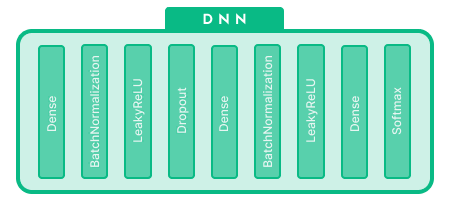
\includegraphics[width=\textwidth]{figures/architecture/DNN.png}
    \caption{Especialista DNN ($\mathcal{E}_{\mathrm{DNN}}$).}
    \label{subfig:arch_dnn}
\end{subfigure}
\hfill
\begin{subfigure}[b]{0.54\textwidth}
    \centering
    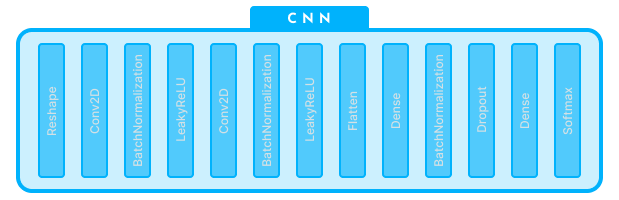
\includegraphics[width=\textwidth]{figures/architecture/CNN.png}
    \caption{Especialista CNN 2D ($\mathcal{E}_{\mathrm{CNN}}$).}
    \label{subfig:arch_cnn}
\end{subfigure}

\vspace{0.3cm}

\begin{subfigure}[b]{0.43\textwidth}
    \centering
    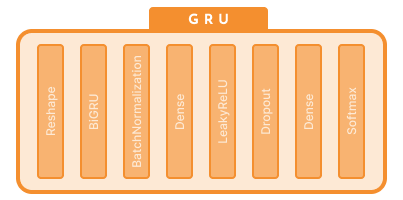
\includegraphics[width=\textwidth]{figures/architecture/GRU.png}
    \caption{Especialista GRU ($\mathcal{E}_{\mathrm{GRU}}$).}
    \label{subfig:arch_gru}
\end{subfigure}
\hfill
\begin{subfigure}[b]{0.53\textwidth}
    \centering
    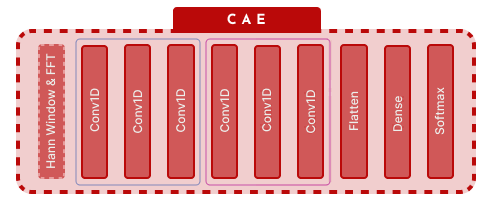
\includegraphics[width=\textwidth]{figures/architecture/CAE.png}
    \caption{Especialista CAE ($\mathcal{E}_{\mathrm{CAE}}$).}
    \label{subfig:arch_cae}
\end{subfigure}

\vspace{0.3cm}

\begin{subfigure}[b]{0.45\textwidth}
    \centering
    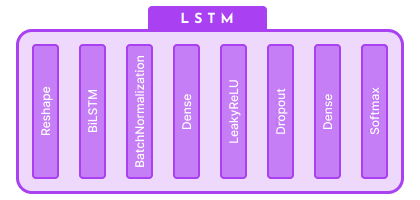
\includegraphics[width=\textwidth]{figures/architecture/LSTM.png}
    \caption{Especialista LSTM ($\mathcal{E}_{\mathrm{LSTM}}$).}
    \label{subfig:arch_lstm}
\end{subfigure}
\fonte{Elaborado pelo autor (2026).}
\end{figure}


\subsection{Gating Network com Refinamento Atencional e Compressão Simétrica}
\label{subsec:gating_network}

A rede de roteamento (\emph{Gating Network}) atua como o árbitro inteligente do comitê de especialistas. Ao contrário de abordagens ensemble com votação estática ou ponderação fixa, a Gating Network inspeciona o vetor completo de telemetria $\mathbf{x} \in \mathbb{R}^{73}$ e calcula dinamicamente a relevância de cada especialista para o fluxo específico sob análise.

Formalmente, a Gating Network processa $\mathbf{x}$ através de duas camadas densas ($128$ e $64$ unidades com Batch Normalization, ativação LeakyReLU com $\alpha=0{,}2$ e Dropout $p=0{,}1$), projetando os logits brutos $\mathbf{z}_{\mathrm{raw}} \in \mathbb{R}^5$, conforme esquematizado na \ref{fig:arch_gating_network}. A distribuição preliminar de confiança $\boldsymbol{\alpha}$ é calculada via Softmax:
\begin{equation}
\label{eq:gating_alpha}
\boldsymbol{\alpha} = \operatorname{softmax}(\mathbf{z}_{\mathrm{raw}}) \in \mathbb{R}^5.
\end{equation}

Em seguida, o vetor $\boldsymbol{\alpha}$ é submetido à camada customizada \texttt{AttentionRefinementLayer}:
\begin{equation}
\label{eq:gating_refinement}
\mathbf{z}_{\mathrm{refined}} = \mathbf{W}_g \ln(\boldsymbol{\alpha} + \epsilon) + \mathbf{b}_g,
\end{equation}
em que $\mathbf{W}_g \in \mathbb{R}^{5 \times 5}$ e $\mathbf{b}_g \in \mathbb{R}^5$ são pesos aprendíveis e $\epsilon = 10^{-7}$ previne instabilidades logarítmicas. Para impedir o colapso e a extinção catastrófica de especialistas (cenário no qual pesos poderiam decair para ordens ínfimas como $10^{-8}$ e desativar especialistas vitais como o CAE), aplica-se a compressão simétrica via tangente hiperbólica:
\begin{equation}
\label{eq:gating_tanh}
\tilde{\mathbf{z}} = \tanh(\mathbf{z}_{\mathrm{refined}}),
\end{equation}
confinando estritamente os logits refinados no intervalo $[-1, 1]$. A distribuição final de pesos atencionais $\mathbf{a}$ é obtida por Softmax temperado:
\begin{equation}
\label{eq:gating_weights}
\mathbf{a} = \operatorname{softmax}\left(\frac{\tilde{\mathbf{z}}}{\tau}\right) = [a_{\mathrm{dnn}}, a_{\mathrm{cnn}}, a_{\mathrm{gru}}, a_{\mathrm{cae}}, a_{\mathrm{lstm}}]^\top,
\end{equation}
em que $\sum_{k=1}^5 a_k = 1$ e $a_k > 0$, mantendo a temperatura inicial calibrada em $\tau = 1{,}0$ \cite{guo2017calibration}.

\begin{figure}[htb]
\centering
\caption{Topologia interna da Gating Network com refinamento atencional e compressão simétrica.}
\label{fig:arch_gating_network}
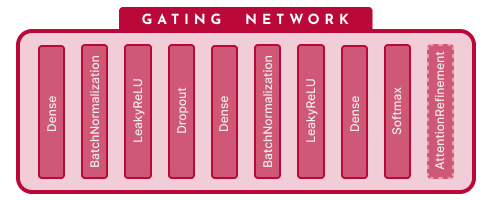
\includegraphics[width=0.75\textwidth]{figures/architecture/GATING_NETWORK.png}
\fonte{Elaborado pelo autor (2026).}
\end{figure}


\subsection{Mecanismo Attention-based Learnable Fusion (ALF)}
\label{subsec:mecanismo_alf}

A integração final das decisões é conduzida pelo módulo customizado \textbf{ALF} (\emph{Attention-based Learnable Fusion}), cuja topologia interna é apresentada na \ref{fig:arch_alf}, estruturado em dois blocos determinísticos:

\begin{enumerate}
    \item \textbf{Fusão Estrita por Soma Ponderada (\texttt{WeightedSumFusion}):}
    A camada de fusão recebe as distribuições probabilísticas preditas por cada um dos cinco especialistas $\{\hat{\mathbf{y}}^{(k)}\}_{k=1}^5 \subset \mathbb{R}^C$ e o vetor de pesos atencionais $\mathbf{a} \in \mathbb{R}^5$ proveniente da Gating Network, efetuando a soma ponderada estrita:
    \begin{equation}
    \label{eq:alf_weighted_sum}
    \mathbf{z} = \sum_{k=1}^5 a_k \cdot \hat{\mathbf{y}}^{(k)} \in \mathbb{R}^C.
    \end{equation}
    Nenhuma conexão residual externa ou concatenação paralela contorna a soma ponderada. Essa decisão de projeto impõe que $100\%$ do fluxo de gradientes retropropagados atravesse a ponderação $a_k \hat{\mathbf{y}}^{(k)}$, forçando a Gating Network a exercer sua função seletiva e incentivando a especialização real de cada rede neural;
    
    \item \textbf{Cabeça Profunda de Decisão Multiclasse:}
    O vetor fundido $\mathbf{z}$ é subsequentemente processado por uma cabeça classificadora profunda desenhada para refinar as margens de decisão entre classes com alta sobreposição:
    \begin{align}
    \label{eq:alf_deep_head_1}
    \mathbf{u}_1 &= \operatorname{LeakyReLU}_{0{,}2}(\operatorname{BN}(\mathbf{W}_1 \mathbf{z} + \mathbf{b}_1)) \in \mathbb{R}^{128}, \\
    \mathbf{u}_1^{\mathrm{drop}} &= \operatorname{Dropout}_{0{,}1}(\mathbf{u}_1), \\
    \mathbf{u}_2 &= \operatorname{LeakyReLU}_{0{,}2}(\operatorname{BN}(\mathbf{W}_2 \mathbf{u}_1^{\mathrm{drop}} + \mathbf{b}_2)) \in \mathbb{R}^{64}, \\
    \label{eq:saida_alf_softmax}
    \hat{\mathbf{y}}_{\mathrm{ALF}} &= \operatorname{softmax}(\mathbf{W}_3 \mathbf{u}_2 + \mathbf{b}_3) \in \mathbb{R}^C.
    \end{align}
\end{enumerate}

\begin{figure}[htb]
\centering
\caption{Topologia interna do módulo de fusão ALF (\emph{Attention-based Learnable Fusion}).}
\label{fig:arch_alf}
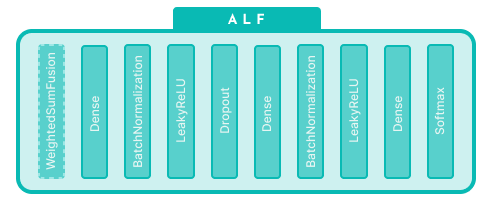
\includegraphics[width=0.75\textwidth]{figures/architecture/ALF.png}
\fonte{Elaborado pelo autor (2026).}
\end{figure}

A arquitetura macroscópica unificada do modelo ALF-MoE, integrando a recepção da telemetria de rede, o roteamento pelos especialistas heterogêneos, a arbitragem dinâmica pela Gating Network e a combinação ponderada das probabilidades com refinamento profundo no módulo ALF, é ilustrada na \ref{fig:arch_alf_moe}.

\begin{figure}[htb]
\centering
\caption{Visão arquitetural integrada do modelo ALF-MoE, evidenciando o fluxo de tensores entre especialistas, Gating Network e fusão ALF.}
\label{fig:arch_alf_moe}
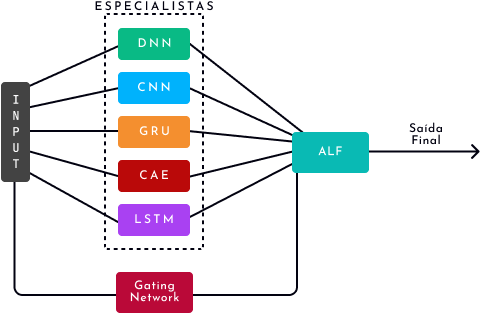
\includegraphics[width=0.75\textwidth]{figures/architecture/ALF-MoE.png}
\fonte{Elaborado pelo autor (2026).}
\end{figure}


\section{Protocolo Experimental de Treinamento e Avaliação}
\label{sec:protocolo_experimental}

Para garantir rigor metodológico e reprodutibilidade, todos os ensaios foram balizados por um protocolo padronizado de otimização multitarefa, particionamento e validação estatística.

\subsection{Funções de Perda e Otimização Multitarefa}
\label{subsec:funcoes_perda}

O treinamento do modelo ALF-MoE é formulado como uma otimização multitarefa conjunta (\emph{multi-task learning}). A função de custo global $\mathcal{L}_{\mathrm{total}}$ agrega a perda da cabeça principal de fusão ALF, as perdas supervisionadas auxiliares dos cinco especialistas e a perda mista de reconstrução espectral do Autoencoder Convolucional:
\begin{equation}
\label{eq:perda_multitarefa}
\mathcal{L}_{\mathrm{total}} = 1{,}0 \cdot \mathcal{L}_{\mathrm{FL}}(\hat{\mathbf{y}}_{\mathrm{ALF}}, \mathbf{y}) + 0{,}2 \sum_{k=1}^5 \mathcal{L}_{\mathrm{FL}}(\hat{\mathbf{y}}^{(k)}, \mathbf{y}) + \lambda_{\mathrm{rec}} \mathcal{L}_{\mathrm{CAE,rec}},
\end{equation}
sendo $\lambda_{\mathrm{rec}} = 1{,}0$ e o peso das cabeças auxiliares fixado em $0{,}2$, provendo sinal de gradiente para guiar os especialistas sem sobrecarregar a convergência da cabeça unificada ALF.

A perda de classificação empregada em todas as cabeças é a \textbf{Focal Loss Multiclasse} \cite{lin2017focal}, definida por:
\begin{equation}
\label{eq:focal_loss}
\mathcal{L}_{\mathrm{FL}}(p_t) = -\alpha_t (1 - p_t)^\gamma \ln(p_t),
\end{equation}
em que $p_t$ representa a probabilidade estimada pelo modelo para a classe verdadeira, $\gamma = 2{,}0$ atua como o parâmetro de foco que suprime gradientes de exemplos fáceis e bem classificados, e $\alpha_t = w_c$ corresponde aos pesos balanceados por raiz quadrada definidos na Equação~\ref{eq:class_weights}.

O otimizador utilizado é o \textbf{Adam} com taxa de aprendizado inicial $\eta_0 = 10^{-3}$, momentos $\beta_1 = 0{,}9$, $\beta_2 = 0{,}999$, $\epsilon = 10^{-8}$ e tamanho de lote (\emph{batch size}) fixado em $128$ instâncias ao longo de $10$ épocas. O agendamento da taxa de aprendizado é governado pelo mecanismo \texttt{ReduceLROnPlateau} (fator de redução $0{,}5$, paciência de $2$ épocas monitorando \texttt{val\_ALF\_F1-Score} com limiar inferior de $10^{-6}$), complementado por parada precoce (\texttt{EarlyStopping}) com paciência de $4$ épocas monitorando a mesma métrica.


\subsection{Métricas de Avaliação}
\label{subsec:metricas_avaliacao}

A avaliação de desempenho do modelo e de cada especialista individual engloba métricas de eficácia preditiva e métricas de eficiência computacional em tempo de execução.

\subsubsection{Métricas de Eficácia Estatística}

Para cada classe $c \in \{0, \dots, C-1\}$, denotam-se $TP_c, FP_c, FN_c, TN_c$ os quantitativos de verdadeiros positivos, falsos positivos, falsos negativos e verdadeiros negativos, respectivamente. Computam-se:
\begin{enumerate}
    \item \textbf{Acurácia Global ($\mathrm{Acc}$):}
    \begin{equation}
    \mathrm{Acc} = \frac{\sum_{c=0}^{C-1} TP_c}{\sum_{c=0}^{C-1} (TP_c + FN_c)};
    \end{equation}
    
    \item \textbf{Acurácia Balanceada ($\mathrm{Acc}_{\mathrm{bal}}$):} média aritmética das taxas de recall sobre todas as classes, mitigando a distorção induzida por classes majoritárias:
    \begin{equation}
    \mathrm{Acc}_{\mathrm{bal}} = \frac{1}{C} \sum_{c=0}^{C-1} \frac{TP_c}{TP_c + FN_c};
    \end{equation}
    
    \item \textbf{Precisão Macro ($\mathrm{Prec}_{\mathrm{macro}}$) e Sensibilidade Macro ($\mathrm{Rec}_{\mathrm{macro}}$):}
    \begin{equation}
    \mathrm{Prec}_{\mathrm{macro}} = \frac{1}{C} \sum_{c=0}^{C-1} \frac{TP_c}{TP_c + FP_c}, \quad \mathrm{Rec}_{\mathrm{macro}} = \frac{1}{C} \sum_{c=0}^{C-1} \frac{TP_c}{TP_c + FN_c};
    \end{equation}
    
    \item \textbf{Macro $F_1$-Score ($F_1^{\mathrm{macro}}$):} média harmônica entre precisão e sensibilidade computada de forma não ponderada, constituindo o critério primordial para ranqueamento de NIDS sob desbalanceamento:
    \begin{equation}
    F_1^{\mathrm{macro}} = \frac{1}{C} \sum_{c=0}^{C-1} \frac{2 \cdot \mathrm{Prec}_c \cdot \mathrm{Rec}_c}{\mathrm{Prec}_c + \mathrm{Rec}_c};
    \end{equation}
    
    \item \textbf{Weighted $F_1$-Score ($F_1^{\mathrm{weighted}}$):} ponderação das pontuações $F_1$ pela proporção empírica de amostras de cada classe $N_c / N$.
\end{enumerate}

\subsubsection{Métricas de Eficiência Computacional}

A viabilidade de implantação do NIDS em nós de monitoramento em tempo real depende estritamente do tempo de processamento. Avaliam-se:
\begin{enumerate}
    \item \textbf{Latência por Amostra ($L_{\mathrm{sample}}$):} tempo médio transcorrido para inferir um único fluxo de rede, expresso em milissegundos por fluxo ($\mathrm{ms/fluxo}$):
    \begin{equation}
    L_{\mathrm{sample}} = \frac{T_{\mathrm{total,inf}}}{N_{\mathrm{test}}} \times 10^3;
    \end{equation}
    
    \item \textbf{Vazão de Inferência ($\mathrm{Throughput}$):} taxa de processamento sustentada expressa em fluxos por segundo ($\mathrm{fluxos/s}$):
    \begin{equation}
    \mathrm{Throughput} = \frac{N_{\mathrm{test}}}{T_{\mathrm{total,inf}}}.
    \end{equation}
\end{enumerate}
